%-------------------------------------------------------------------------------
\section{Einführung in die Vorlesung}
%-------------------------------------------------------------------------------

%%% Folie
\begin{frame}{Kompetenzziele der Vorlesung}
    \begin{itemize}
        \item \textbf{Fachkompetenz:} Die Studierenden kennen den
        \textcolor{NavyBlue}{technischen Aufbau typischer Devices/Embedded Systems}
        im Kontext des Internet of Things. Sie sind in der Lage, entsprechende Devices
        für einen gegebenen Einsatzzweck auszuwählen und zu programmieren.
        \medskip

        \item \textbf{Methodenkompetenz:} Die Studierenden sind in der Lage
        bei der Programmierung von IoT-Geräten systematisch und methodisch vorzugehen.
        \medskip

        \item \textbf{Personale und soziale Kompetenz:} Die Studierenden verstehen die Herausforderungen
        des IoT für Unternehmen, Politik und Gesellschaft und sind in der Lage, diese kompetent zu diskutieren.
        \medskip

        \item \textbf{Übergreifende Handlungskompetenz:} Die Studierenden können reale betriebliche
        Problemstellungen im Kontext von IoT analysieren, \textcolor{NavyBlue}{Konzepte entwerfen}
        und \textcolor{NavyBlue}{IoT-fähige Geräte programmieren} und im Unternehmenskontext integrieren.
        \medskip
    \end{itemize}
\end{frame}

{
\footnotesize
%%% Folie
\begin{frame}{Inhalte der Vorlesung}
        \begin{columns}
            \begin{column}[T]{.5\textwidth}
                \begin{block}{3. Semester}
                    \medskip

                    \begin{enumerate}
                        \item Grundlagen des Internet of Things
                        \item Einführung in Python
                        \item IoT-Entwicklung mit Python
                        \item \textcolor{gray}{Übungsstunde}
                        \item Elektronik für eingebettete Systeme I
                        \item Elektronik für eingebettete Systeme II
                        \item Analoge und digitale Schnittstellen
                        \item \textcolor{gray}{Übungsstunde}
                        \item \textcolor{gray}{Klausurvorbereitung}
                    \end{enumerate}

                    \medskip
                    \textbf{Prüfungsform:} Klausur
                \end{block}
            \end{column}
            \begin{column}[T]{.5\textwidth}
                \begin{block}{4. Semester}
                    \medskip

                    \begin{enumerate}
                        \item Wiederholung und Ausblick
                        \item Python-Architekturmuster für IoT-Devices
                        \item Vorstellung der Referenzarchitektur I
                        \item Vorstellung der Referenzarchitektur II
                        \item Hardwaredesign und Prototyping
                        \item \textcolor{gray}{Assignment}
                        \item \textcolor{gray}{Assignment}
                        \item \textcolor{gray}{Assignment}
                        \item \textcolor{gray}{Assignment}
                    \end{enumerate}

                    \medskip
                    \textbf{Prüfungsform:} Assignment
                \end{block}
            \end{column}
        \end{columns}
\end{frame}
}

%%% Folie
\begin{frame}{Vorausgesetztes Wissen}
    \begin{columns}
        \column{\dimexpr\paperwidth-10pt}
        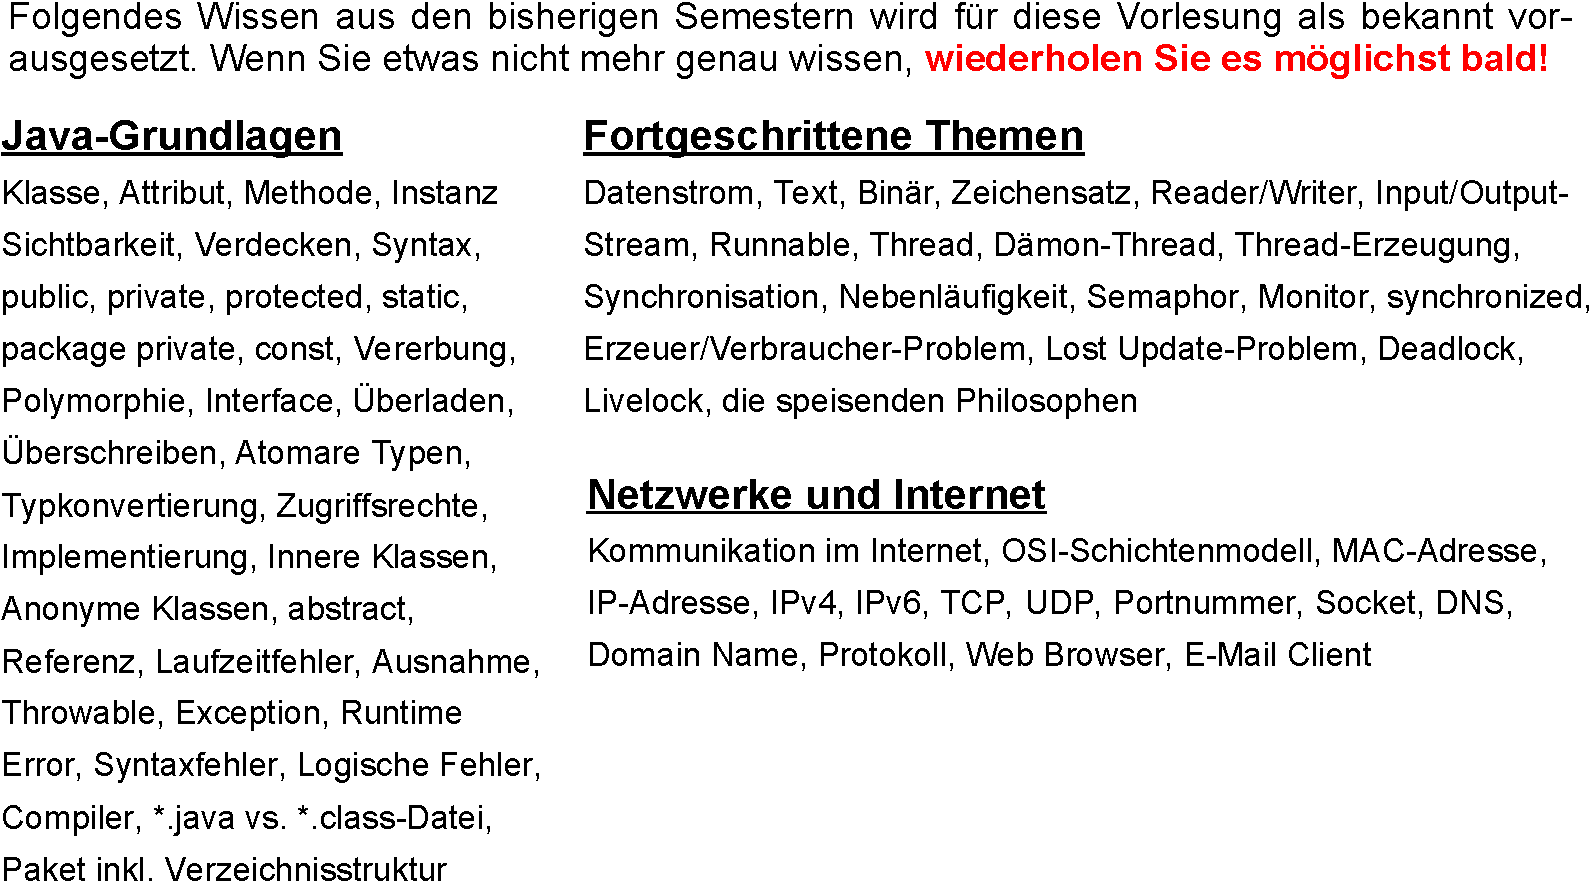
\includegraphics[width=\textwidth]{img/vorausgesetztes_wissen}
    \end{columns}
\end{frame}


%%% Folie
\begin{frame}{Benötigte Hard- und Software}
        \begin{columns}
            \begin{column}[T]{.5\textwidth}
                \textbf{Hardware}
                \medskip

                \Justified{
                    \footnotesize
                    Kann im WWI-Labor für die Dauer des Moduls kostenlos ausgeliehen
                    werden. Rückgabe am Ende des vierten Semesters, da dieselbe
                    Hardware dann direkt für das IoT-Integrationsseminar und Projekt
                    benötigt wird.
                }
                \medskip

                \begin{itemize}
                    \item Raspberry Pi
                    \item Diverse Sensoren und Aktoren
                \end{itemize}
            \end{column}
            \begin{column}[T]{.5\textwidth}
                \textbf{Software}
                \medskip

                \Justified{
                    \footnotesize
                    Lediglich ein paar Entwicklungswerkzeuge für die Programmierung mit
                    Python sowie die Remote-Entwicklung werden benötigt. Einige Beispiele
                    können auch lokal ohne Raspberry Pi ausgeführt werden, wofür auf Ihrem
                    Laptop ebenfalls Python benötigt wird.
                }
                \medskip

                \begin{itemize}
                    \item Visual Studio Code
                    \item OpenSSH
                    \item Python
                    \item KiCAD (optional)
                \end{itemize}
            \end{column}
        \end{columns}

        \bigskip

        \Justified{
            \scriptsize
            \textcolor{gray}{
                Python werden wir verwenden, um den Raspberry Pi zu programmieren. Zum Einstieg
                in die Sprache kann es ganz sinnvoll sein, den Python-Interpreter zusätzlich auf
                dem eigenen Laptop zu installieren. KiCAD benötigen Sie nur, wenn Sie im Kapitel
                über Hardwaredesign das Fallbeispiel zum Entwurf eigener Schaltungen nachvollziehen
                wollen.
            }
        }
\end{frame}

%%% Folie
{
\footnotesize
\setlength{\fboxsep}{0pt}

\begin{frame}{Literaturempfehlungen}
    \fbox{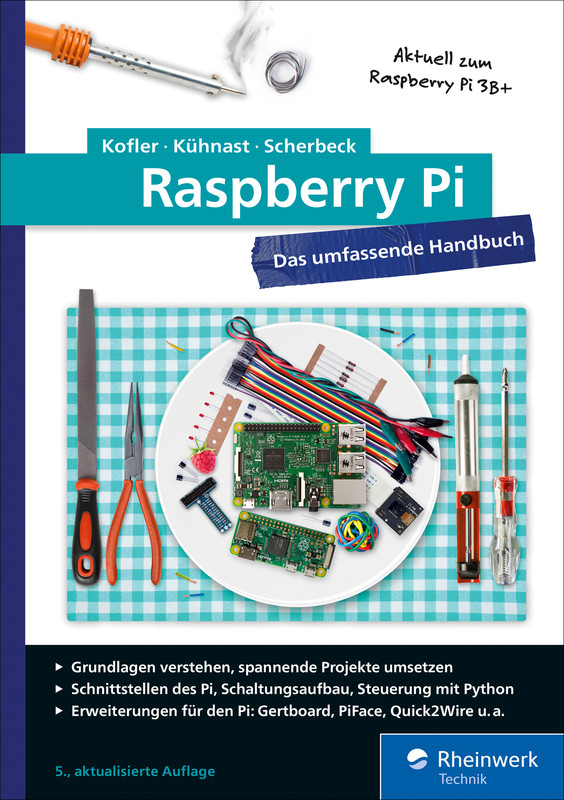
\includegraphics[height=3.3cm]{img/buch_raspberrypi}}
    \hfill
    \fbox{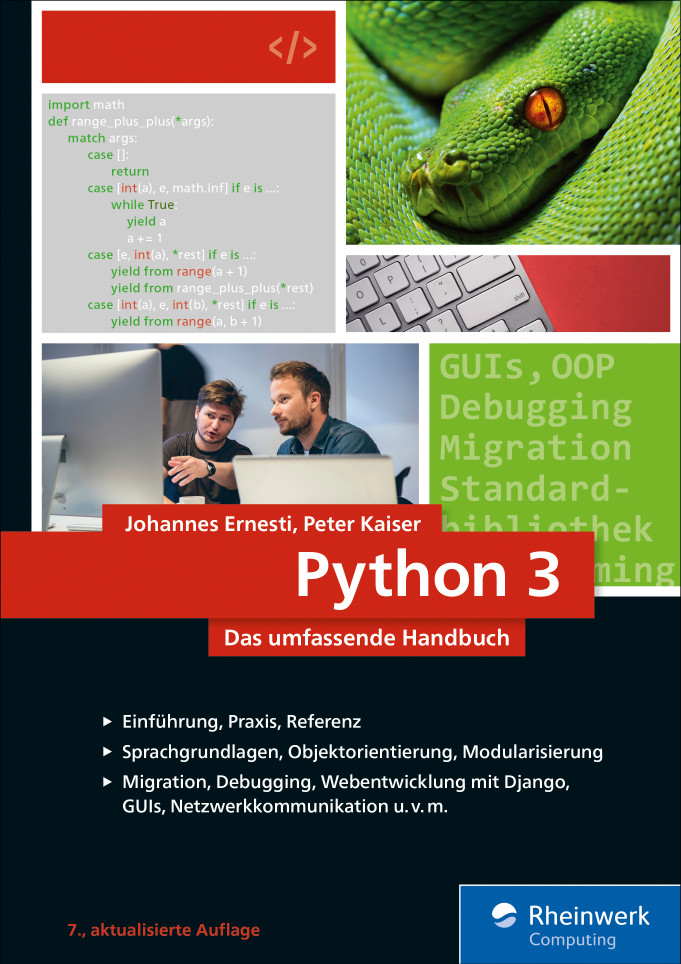
\includegraphics[height=3.3cm]{img/buch_python3_handbuch}}
    \hfill
    \fbox{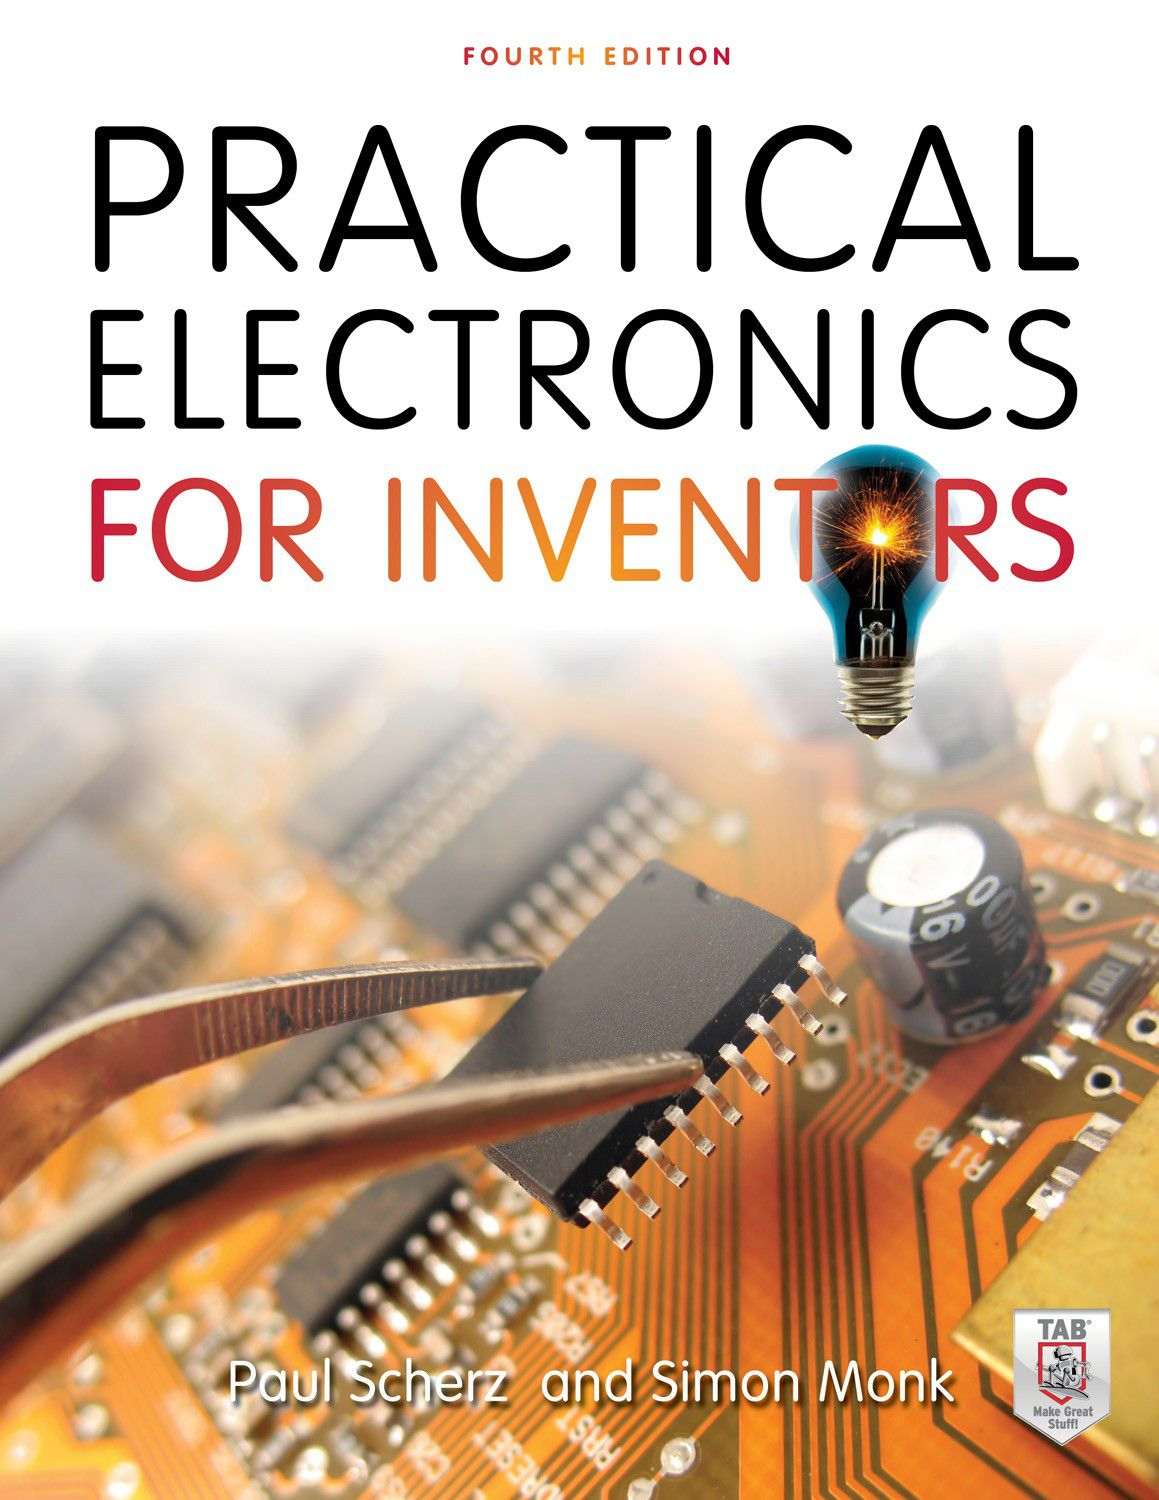
\includegraphics[height=3.3cm]{img/buch_practical_electronics}}
    \hfill
    \fbox{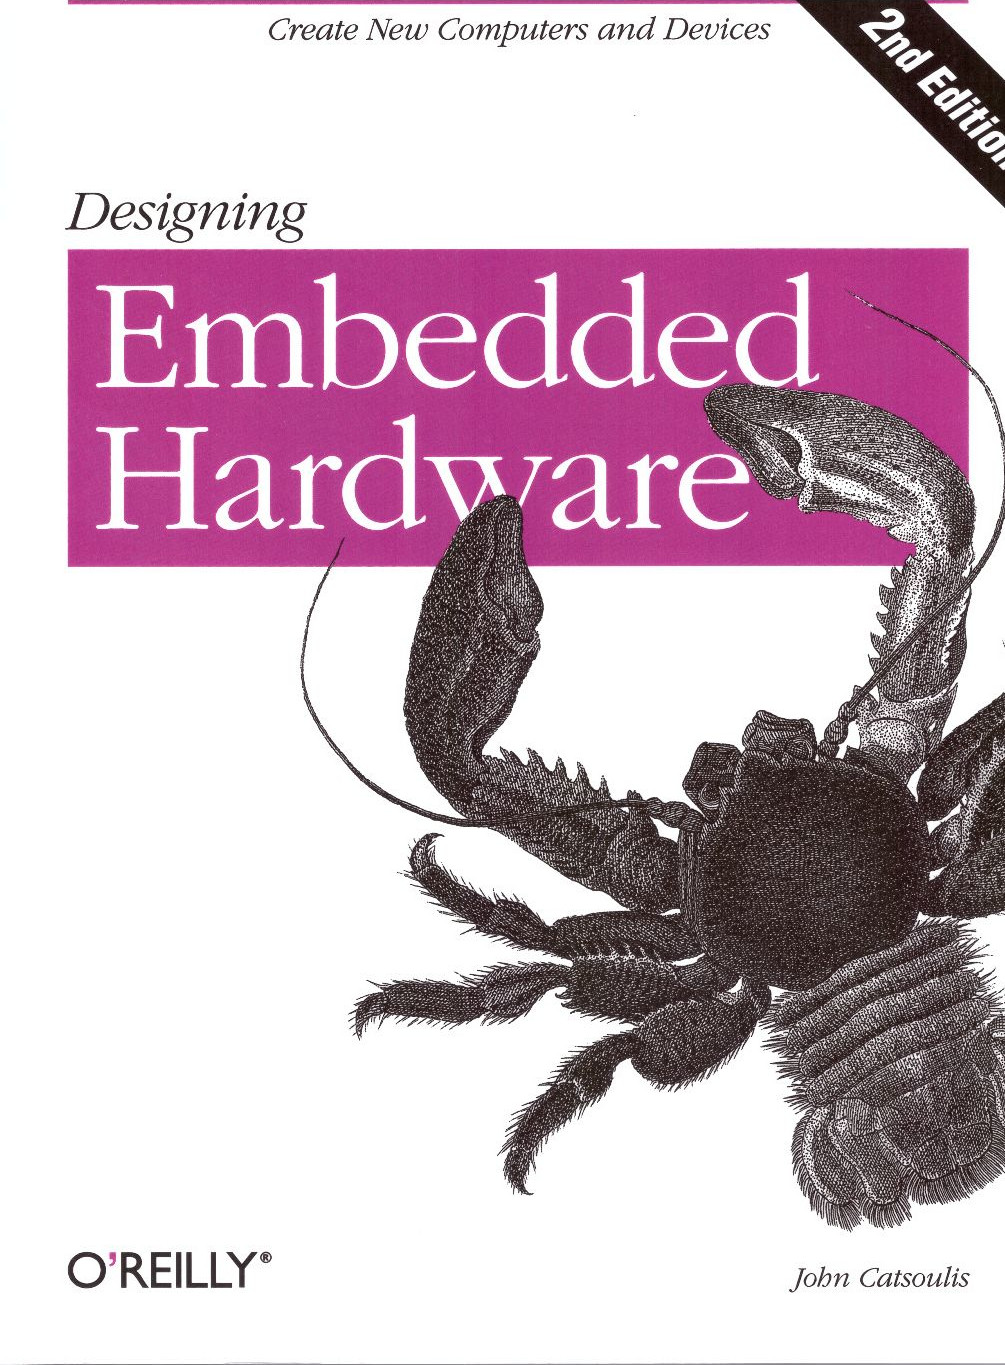
\includegraphics[height=3.3cm]{img/buch_embedded_hardware}}

    \vskip 0.6cm

    \begin{columns}
        \column[T]{.5\textwidth}
        \textbf{Raspberry Pi: Das umfassende Handbuch} \\ Rheinwerk Verlag, 2018

        \column[T]{.5\textwidth}
        \textbf{Python 3: Das umfassende Handbuch} \\ Rheinwerk Verlag, 2023
    \end{columns}

    \vskip 0.6cm

    \begin{columns}
        \column[T]{.5\textwidth}
        \textbf{Practical Electronics for Inventors} \\ McGraw-Hill, 2016

        \column[T]{0.5\textwidth}
        \textbf{Designing Embedded Hardware} \\ O'Reilly, 2005
    \end{columns}
\end{frame}
}
